\documentclass[11pt]{article}
\usepackage[hmargin=1in,vmargin=1in]{geometry}
\usepackage{xcolor}
\usepackage{amsmath,amssymb,amsfonts,url,sectsty,framed,tcolorbox,framed}
\usepackage{nicematrix}
\usepackage{tikz}
\newcommand{\pf}{{\bf Proof: }}
\newtheorem{theorem}{Theorem}
\newtheorem{lemma}{Lemma}
\newtheorem{proposition}{Proposition}
\newtheorem{definition}{Definition}
\newtheorem{remark}{Remark}
\newcommand{\qed}{\hfill \rule{2mm}{2mm}}


\begin{document}
%%%%%%%%%%%%%%%%%%%%%%%%%%%%%%%%%%%%%%%%%%%%%%%%%%%%%%%%%%%%%%%%%%%%%
\noindent
\rule{\textwidth}{1pt}
\begin{center}
{\bf [CS304] Introduction to Cryptography and Network Security}
\end{center}
Course Instructor: Dr. Dibyendu Roy \hfill Winter 2022-2023\\
Scribed by: Archit Agrawal (202051213) \hfill Lecture 3 and 4 (Week 2)
\\
\rule{\textwidth}{1pt}
%%%%%%%%%%%%%%%%%%%%%%%%%%%%%%%%%%%%%%%%%%%%%%%%%%%%%%%%%%%
%write here

\section{Quick Recap}
In the first week, the following topics were covered:
\begin{itemize}
    \item Cryptography, Cryptanalysis and Cryptology
    \item Encryption and Decryption
    \item Types of Cryptography: Symmetric and Asymmetric Cryptography
    \item Security Services
    \item Functions: One-One, Onto, Bijection, Permutation, One-Way, Substitution Box
    \item Classical Ciphers: Caesar, Transposition, Substitution, Affine and Playfair (Encryption only)
    \item Basic Mathematics: Multiplicative Inverse in Modular Arithmetic, Euler's Totient Function and Extended Euclidean Algorithm
\end{itemize}

\section{Classical Ciphers}
\subsection{Playfair Cipher}
Playfair Cipher uses a 5 $\times$ 5 matrix formed using the secret key for encryption and decryption.\\
\newline
\textbf{Encryption:} The following rules are followed for encryption:
\begin{enumerate}
    \item Create the 5 $\times$ 5 matrix using secret key.Rules for creating the matrix are mentioned below:
    \begin{itemize}
        \item Characters I and J are considered as same.
        \item Fill the key characters row-wise in the matrix. If a character has already appeared, skip it.
        \item Fill the remaining alphabets in lexicographic order.
    \end{itemize}
    \item Break the message (plain text) into groups of 2 characters.
    \item Add fillers if a group has same characters or if it has only one character.
    \begin{itemize}
        \item If length of message is odd, add X at the end of message. For example:
        \begin{center}
            Plain Text: CSE\\
            After Insertion: CS EX
        \end{center}
        \item If both the characters are same, add an X after the first character. For Example:
        \begin{center}
            Plain Text: BALL\\
            After Insertion: BA LX LX
        \end{center}
    \end{itemize}
    \item For each group, find the characters in the matrix. Do the following according to the position of these characters:
    \begin{itemize}
        \item If both characters are in the same row, use the next right character as cipher text. If the plain text character is the last element of that row,  take the first character of that row as cipher text.
        \item If both characters are in the same column, use the next down character as cipher text. If the plain text character is the last element of that column, take the first character of that column as cipher text.
        \item If the characters are in different rows and columns, form a rectangle with these two characters at corners. Now, use the other row corner as the cipher text for both characters.
    \end{itemize}
\end{enumerate}

\textbf{Example 1:}
\begin{center}
    Secret Key: PLAYFAIR EXAMPLE\\
    Plain Text: HIDE\\
\end{center}
The matrix formed using encryption rules will be:
\begin{center}
    \begin{bmatrix}
    P & L & A & Y & F\\
    I & R & E & X & M\\
    B & C & D & G & H\\
    K & N & O & Q & S\\
    T & U & V & W & Z\\
    \end{bmatrix}
\end{center}
Now, breaking the plain text into groups of 2 will give us:
\begin{center}
    Plain Text: HI DE
\end{center}
\begin{center}
    $\begin{pNiceMatrix}[margin]
    P & L & \Block[draw,fill=green!15,rounded-corners]{5-1}{} A & Y & F \\
    \Block[draw,fill=red!15,rounded-corners]{2-5}{}
    I & R & E & X & M \\
    B & C & D & G & H \\
    K & N & O & Q & S \\
    T & U & V & W & Z \\
    \end{pNiceMatrix}$
\end{center}
For the first group, the characters H and I form a rectangle shown by red colour in the figure above. Hence, the corners will be swapped.
\begin{center}
    Plain Text: HI DE\\
    Cipher Text: BM OD
\end{center}
For the second group, the characters D and E are in the same column. Hence, the next down character will be the cipher text.
\newline


\textbf{Decryption:} The following rules are followed for decryption:
\begin{enumerate}
    \item The first two rules, that is, the matrix construction and breaking the cipher text into groups of two is same as done during encryption.
    \item For each group of cipher text, find the characters in the matrix. Do the following according to the position of these characters:
    \begin{itemize}
        \item If both characters are in the same row, use the next left character as plain text. If the cipher text character is the last element of that row,  take the first character of that row as plain text.
        \item If both characters are in the same column, use the next upper character as plain text. If the cipher text character is the last element of that column, take the first character of that column as plain text.
        \item If the characters are in different rows and columns, form a rectangle with these two characters at corners. Now, use the other row corner as the plain text for both characters.
    \end{itemize}
\end{enumerate}

\textbf{Example 1:}
\begin{center}
    Secret Key: PLAYFAIR EXAMPLE\\
    Cipher Text: BMOD\\
\end{center}
Since the key is same as the encryption example, the matrix will be same as before.\\
Now, breaking the cipher text into groups of 2 will give us:
\begin{center}
    Cipher Text: BM OD
\end{center}
For the first group, the characters B and M form a rectangle shown by red colour in Figure 1. Hence, the corners will be swapped.
\begin{center}
    Cipher Text: BM OD\\
    Cipher Text: HI DE
\end{center}
For the second group, the characters O and D are in the same column. Hence, the next upper character will be the cipher text.

\subsection{Hill Cipher}
In Hill Cipher, the secret key is a $n \times n$ invertible matrix A.
\begin{center}
    A = $(a_{ij})_{n \times n}$ $\rightarrow$ Secret Key
\end{center}
where $a_{ij} \in Z_{26}$.
\begin{center}
    $M = m_1m_2....m_n$ $\rightarrow$ Plain Text \in$ Z_{26}^n$
\end{center}
\textbf{Encryption:}
\begin{center}
    $C = A \cdot M = c_1c_2....c_n$
\end{center}
\textbf{Decryption:}
\begin{center}
    $M = A^{-1} \cdot C$
\end{center}
The inverse of matrix A is given as:
\begin{center}
    $A^{-1} = \frac {1}{|A|} \cdot adj(A)$
\end{center}
where $|A|$ is determinant of A and adj(A) is adjoint of matrix A.\\
While calculating inverse of matrix A during decryption, all the calculations should be done under modulo 26.

\subsection{Substitution Cipher}
Substitution Cipher is a substitution from the set of alphabets to itself. The substitution need not be a bijection.
\begin{center}
    S: \{A,B.....,Z\} $\rightarrow$ \{A,B.....,Z\} \\
    Cipher Text = S(Plain Text)
\end{center}
S is the secret key. The number of secret keys possible is:
\begin{center}
    $\#S = 26^{26} \approx 2^{122}$
\end{center}
If the substitution box S is constrained to be a bijection, then the number of possible keys will be:
\begin{center}
    $\#S = 26!$
\end{center}
Brute Force Attack or Exhaustive Search is a way of finding the plain text if cipher text is known by exhaustively using all the possible keys.

\section{Kerkchoff's Principle}
Kerckhoffs's principle of cryptography was stated by Dutch-born cryptographer Auguste Kerckhoffs in the 19th century. The principle holds that a cryptographic system should be designed to be secure, even if everything about the system, except the key, is publicly known.
\begin{itemize}
    \item The algorithms are designed for a whole lot of people, hence, if the design is not public, then people will not be able to use the algorithm.
    \item Another thing is that if one is not sharing their algorithm publicly, then there are more chances of having security weaknesses in the algorithm. Every person can interpret and cryptanlayse the algorithm differently to find security flaws. These flaws can be mitigated to make the algorithm more secure.
\end{itemize}

\section{Shannon's Notion of Perfect Secrecy}
Let E be the encryption algorithm, M be the plain text and C be the cipher text. Hence,
\begin{center}
    C = E(M)
\end{center}

%The main motivation of cryptographic systems is that from the cipher text, no one can get the original message
Perfect Secrecy is the notion that given an encrypted message from a perfectly secure encryption system, absolutely nothing will be revealed about the unencrypted message from the cipher text. No information means not even a single bit of message or a function on any single bit of message is revealed.\\ For Example, suppose a single bit message is encrypted using some algorithm. The probability distribution of the message is given in Table 1.
\begin{table}[h]
\centering
\begin{tabular}{l|r}
Value & $P(n)$ \\\hline
0 & 0.9 \\
1 & 0.1
\end{tabular}
\caption{\label{tab:widgets} Probability Distribution.}
\end{table}
An algorithm will be perfectly secure if from the encrypted message, the probability of guessing the plain text as 0 is not (0.9 + $\epsilon)$ where $\epsilon > 0.$\\
The notion of perfect secrecy can be represented mathematically as:
\begin{center}
    $Pr[M=m|C=c] = Pr[M=m]$\\
    $Pr[message | cipher text] = Pr[message]$
\end{center}
There are certain algorithms which provide perfect secrecy following some limitations. However, with these limitations these algorithms are impractical and cannot be used. One such algorithm is One Time Padding(OTP). 

\section{Symmetric Key Cipher}
It has one secret key for both encryption and decryption functions. Since the key for both encryption and decryption is same, no one else should know about the key other than the sender and the receiver. There are two different types of Symmetric Key Ciphers:
\begin{enumerate}
    \item Block Cipher
    \item Stream Cipher
\end{enumerate}

\subsection{Block Cipher}
The message to be encrypted is divided into fixed length blocks and these blocks are encrypted, that is, the encryption is done in block-wise manner. For example, the DES algorithm can encrypt 64 bit messages.
\begin{center}
    $M = m_o||m_1||....||m_n$\\
    length of block = l\\
    $m_0, m_1, ..., m_n$ are blocks of length l
\end{center}
One way of encrypting block-wise is to encrypt each block and then concatenate each block in the same order.
\begin{center}
    $M = m_0 || m_1 || .... || m_n$ \\
    $C = Enc(m_0, K) || Enc(m_1, K) || .... || Enc(m_n, K)$ \\
    $C = C_0 || C_1 || .... || C_n$
\end{center}
It is not necessary that these blocks will be concatenated just as they were in the original message. There can be some algorithm for mixing these blocks and generating the encrypted text.\\
\newline
All the block ciphers are designed using either Substituion Permutation Networks or Feistel Networks. The AES algorithm is based on Substituion Permutation Networks and the DES algorithm is based on Fiestel Networks.

\subsection{Stream Cipher}
The encryption in Stream Cipher is done bit-wise. The message is a bit stream represented as:
\begin{center}
    $M = m_0m_1...m_l,$ where $ m_i \in {0, 1}$
\end{center}
An algorithm will be used to generate another bit stream represented as:
\begin{center}
    $Z = Z_0Z_1...Z_l,$ where $ Z_i \in {0, 1}$
\end{center}
This bit stream can be the output of a function which takes key and message as input.\\
To generate the cipher text, XOR between bits of plain text and bits of Z will be performed.
\begin{center}
    $C = (m_0 \oplus Z_0, m_1 \oplus Z_1,...., m_l \oplus Z_l)$
\end{center}
During decryption, the same bit stream Z will be generated using the function and XOR will be performed to get the original message. It should be noted that XOR is used here for the sake of example, it can be some other complex computation too.\\

\subsection{Stream Ciphers Versus Block Ciphers}
There are known algorithms which can generate $2^{80} - 1$ bit long bit stream by taking 80 bit key as an input. Hence, using stream cipher, very long messages can be encrypted. However, this is not the case with block ciphers. Suppose an algorithm that encrypts 64 bit blocks at a time. Hence, to encrypt the whole message using block cipher, it will take $2^{74}$ times the time taken to encrypt one block. Hence, stream ciphers provide efficiency over block ciphers. \\
\newline
However, practically the messages are not very large and there are very good software implementation of block ciphers. Hence, where there are small messages, block ciphers are preferred over stream ciphers.\\
\newline
Stream ciphers are used generally where the length of the message is not pre-determined or there can nothing be said about how long the message will become. For example, voice over telephony, that is, the normal phone call uses stream ciphers as the time for which two people will communicate cannot be judged at the starting of the call.\\
\newline
The implementation of block ciphers in hardware is very poor as it requires a lot of gates. Hence, block ciphers are not implemented in hardware. However, all the existing stream ciphers are efficiently implemented in hardware.

\section{Product Cipher}
A Product Cipher combines two or more transformations in a manner intending that the resulting cipher is more secure than the individual transformations. A Product Cipher can be better than individual transformation in terms of both security and efficiency. One such cipher is a Substitution Permutation Network (SPN).

\subsection{Substitution Permutation Network (SPN)}
It is a product cipher based on a substitution box and a permutation box. Let's assume a message of length $n \cdot r$, a substituion S and a permutation P be defined as:
\begin{center}
    $S: \{0, 1\}^n \rightarrow \{0, 1\}^m$\\
    $P: \{0, 1,..., m\cdot r - 1\} \rightarrow \{0, 1,..., m\cdot r - 1\} $
\end{center}

A SPN can be defined as performing a substitution on r blocks of length n, which will generate a $m \cdot r$ length text. Then, performing a permutation on this $m \cdot r$ length text to get the cipher text.

\begin{center}
    \tikzset{every picture/.style={line width=0.75pt}}      
    
    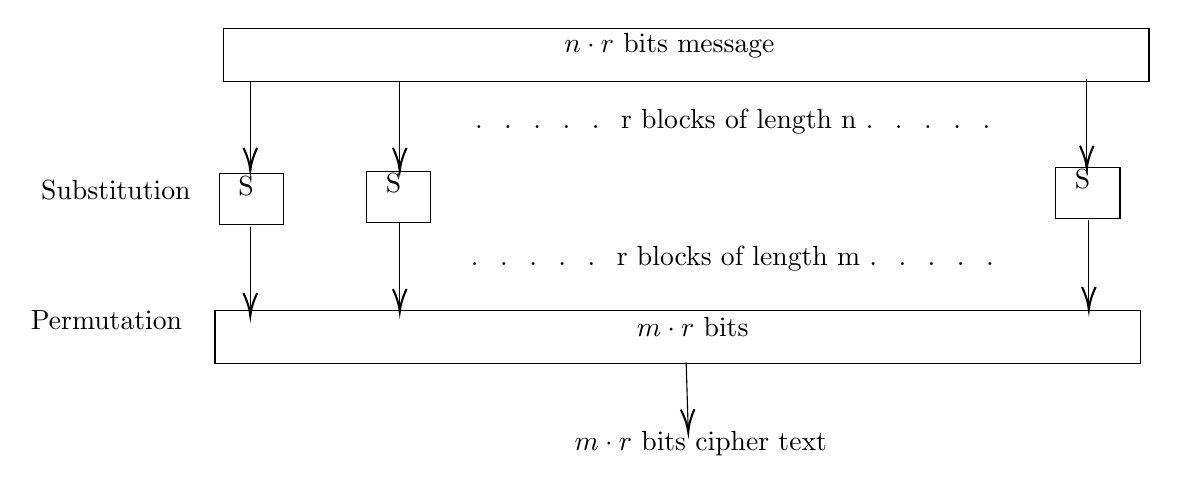
\begin{tikzpicture}[x=0.75pt,y=0.75pt,yscale=-1,xscale=1]
    \draw   (112,21) -- (558,21) -- (558,46.6) -- (112,46.6) -- cycle ;
    \draw    (125,46.6) -- (125,87.6) ;
    \draw [shift={(125,89.6)}, rotate = 270] [color={rgb, 255:red, 0; green, 0; blue, 0 }  ][line width=0.75]    (10.93,-3.29) .. controls (6.95,-1.4) and (3.31,-0.3) .. (0,0) .. controls (3.31,0.3) and (6.95,1.4) .. (10.93,3.29)   ; 
    \draw    (197,46.6) -- (197,87.6) ;
    \draw [shift={(197,89.6)}, rotate = 270] [color={rgb, 255:red, 0; green, 0; blue, 0 }  ][line width=0.75]    (10.93,-3.29) .. controls (6.95,-1.4) and (3.31,-0.3) .. (0,0) .. controls (3.31,0.3) and (6.95,1.4) .. (10.93,3.29)   ;
    \draw    (528,45.6) -- (528,86.6) ;
    \draw [shift={(528,88.6)}, rotate = 270] [color={rgb, 255:red, 0; green, 0; blue, 0 }  ][line width=0.75]    (10.93,-3.29) .. controls (6.95,-1.4) and (3.31,-0.3) .. (0,0) .. controls (3.31,0.3) and (6.95,1.4) .. (10.93,3.29)   ;
    \draw   (110,91) -- (141,91) -- (141,115.6) -- (110,115.6) -- cycle ;
    \draw   (181,90) -- (212,90) -- (212,114.6) -- (181,114.6) -- cycle ;
    \draw   (513,88) -- (544,88) -- (544,112.6) -- (513,112.6) -- cycle ;
    \draw    (125,116.6) -- (125,157.6) ;
    \draw [shift={(125,159.6)}, rotate = 270] [color={rgb, 255:red, 0; green, 0; blue, 0 }  ][line width=0.75]    (10.93,-3.29) .. controls (6.95,-1.4) and (3.31,-0.3) .. (0,0) .. controls (3.31,0.3) and (6.95,1.4) .. (10.93,3.29)   ;
    \draw    (197,114.6) -- (197,155.6) ;
    \draw [shift={(197,157.6)}, rotate = 270] [color={rgb, 255:red, 0; green, 0; blue, 0 }  ][line width=0.75]    (10.93,-3.29) .. controls (6.95,-1.4) and (3.31,-0.3) .. (0,0) .. controls (3.31,0.3) and (6.95,1.4) .. (10.93,3.29)   ; 
    \draw    (529,113.6) -- (529,154.6) ;
    \draw [shift={(529,156.6)}, rotate = 270] [color={rgb, 255:red, 0; green, 0; blue, 0 }  ][line width=0.75]    (10.93,-3.29) .. controls (6.95,-1.4) and (3.31,-0.3) .. (0,0) .. controls (3.31,0.3) and (6.95,1.4) .. (10.93,3.29)   ;
    \draw   (108,157) -- (554,157) -- (554,182.6) -- (108,182.6) -- cycle ;
    \draw    (335,182) -- (335.94,213.6) ;
    \draw [shift={(336,215.6)}, rotate = 268.3] [color={rgb, 255:red, 0; green, 0; blue, 0 }  ][line width=0.75]    (10.93,-3.29) .. controls (6.95,-1.4) and (3.31,-0.3) .. (0,0) .. controls (3.31,0.3) and (6.95,1.4) .. (10.93,3.29)   ;
    
    \draw (275,22) node [anchor=north west][inner sep=0.75pt]   [align=left] {$n \cdot r$ bits message};
    \draw (118,91) node [anchor=north west][inner sep=0.75pt]   [align=left] {S};
    \draw (189,90) node [anchor=north west][inner sep=0.75pt]   [align=left] {S};
    \draw (521,88) node [anchor=north west][inner sep=0.75pt]   [align=left] {S};
    \draw (232,59) node [anchor=north west][inner sep=0.75pt]   [align=left] {. \ . \ . \ . \ . \ r blocks of length n . \ . \ . \ . \ .};
    \draw (230,125) node [anchor=north west][inner sep=0.75pt]   [align=left] {. \ . \ . \ . \ . \ r blocks of length m . \ . \ . \ . \ .};
    \draw (23,93) node [anchor=north west][inner sep=0.75pt]   [align=left] {Substitution};
    \draw (310,159) node [anchor=north west][inner sep=0.75pt]   [align=left] {$m \cdot r$ bits};
    \draw (18,156) node [anchor=north west][inner sep=0.75pt]   [align=left] {Permutation};
    \draw (280,214) node [anchor=north west][inner sep=0.75pt]   [align=left] {$m \cdot r$ bits cipher text};
    \end{tikzpicture}
\end{center}

\section{Feistel Network}
In a Feistel Network, let's say there is a message P of $2n$ bits. This message is divided into two equal parts $L_0$ and $R_0$.
\begin{center}
    P = $L_0 || R_0$.
\end{center}
$L_0$ and $R_0$ are of $n$ bits each and can be calculated using right and left shifting of P by $n$ bits respectively.\\
Let K be the secret key and the length of the secret key be $l$. A fuction f, called as round function, is defined as:
\begin{center}
    $f: \{0, 1\}^n \times \{0, 1\}^l \rightarrow \{0, 1\}^n$
\end{center}
\textbf{Encryption:} The diagram for encryption is given below:

\begin{center}
    \tikzset{every picture/.style={line width=0.75pt}}       
    
    \begin{tikzpicture}[x=0.75pt,y=0.75pt,yscale=-1,xscale=1]
    
    \draw   (127,51.6) -- (261,51.6) -- (261,123) -- (127,123) -- cycle ;
    \draw   (261,51.6) -- (395,51.6) -- (395,123) -- (261,123) -- cycle ;
    \draw   (129,306.6) -- (263,306.6) -- (263,378) -- (129,378) -- cycle ;
    \draw   (263,306.6) -- (397,306.6) -- (397,378) -- (263,378) -- cycle ;
    \draw   (217,151) -- (287,151) -- (287,191) -- (217,191) -- cycle ;
    \draw    (450,158.6) -- (289,158.6) ;
    \draw [shift={(287,158.6)}, rotate = 360] [color={rgb, 255:red, 0; green, 0; blue, 0 }  ][line width=0.75]    (10.93,-3.29) .. controls (6.95,-1.4) and (3.31,-0.3) .. (0,0) .. controls (3.31,0.3) and (6.95,1.4) .. (10.93,3.29)   ;
    \draw    (328,177.6) -- (290,177.98) ;
    \draw [shift={(288,178)}, rotate = 359.43] [color={rgb, 255:red, 0; green, 0; blue, 0 }  ][line width=0.75]    (10.93,-3.29) .. controls (6.95,-1.4) and (3.31,-0.3) .. (0,0) .. controls (3.31,0.3) and (6.95,1.4) .. (10.93,3.29)   ;
     
    \draw    (328.35,124.6) -- (328,177.6) -- (327.64,231.6) -- (190,231.6) -- (191.95,305.6) ;
    \draw [shift={(192,307.6)}, rotate = 268.49] [color={rgb, 255:red, 0; green, 0; blue, 0 }  ][line width=0.75]    (10.93,-3.29) .. controls (6.95,-1.4) and (3.31,-0.3) .. (0,0) .. controls (3.31,0.3) and (6.95,1.4) .. (10.93,3.29)   ;
     
    \draw    (146,124.6) -- (146,150.6) ;
    \draw [shift={(146,152.6)}, rotate = 270] [color={rgb, 255:red, 0; green, 0; blue, 0 }  ][line width=0.75]    (10.93,-3.29) .. controls (6.95,-1.4) and (3.31,-0.3) .. (0,0) .. controls (3.31,0.3) and (6.95,1.4) .. (10.93,3.29)   ;
    
    \draw   (134,167.3) .. controls (134,159.18) and (139.37,152.6) .. (146,152.6) .. controls (152.63,152.6) and (158,159.18) .. (158,167.3) .. controls (158,175.42) and (152.63,182) .. (146,182) .. controls (139.37,182) and (134,175.42) .. (134,167.3) -- cycle ; \draw   (134,167.3) -- (158,167.3) ; \draw   (146,152.6) -- (146,182) ;
    
    \draw    (217,168.6) -- (160,167.34) ;
    \draw [shift={(158,167.3)}, rotate = 1.26] [color={rgb, 255:red, 0; green, 0; blue, 0 }  ][line width=0.75]    (10.93,-3.29) .. controls (6.95,-1.4) and (3.31,-0.3) .. (0,0) .. controls (3.31,0.3) and (6.95,1.4) .. (10.93,3.29)   ;
    
    \draw    (146,182) -- (146,244.6) -- (325.01,242.74) -- (325.97,305.6) ;
    \draw [shift={(326,307.6)}, rotate = 269.13] [color={rgb, 255:red, 0; green, 0; blue, 0 }  ][line width=0.75]    (10.93,-3.29) .. controls (6.95,-1.4) and (3.31,-0.3) .. (0,0) .. controls (3.31,0.3) and (6.95,1.4) .. (10.93,3.29)   ;
    
    
    \draw (180,75) node [anchor=north west][inner sep=0.75pt]   [align=left] {$L_0$};
    \draw (316,75) node [anchor=north west][inner sep=0.75pt]   [align=left] {$R_0$};
    \draw (318,331) node [anchor=north west][inner sep=0.75pt]   [align=left] {$R_1$};
    \draw (180,327) node [anchor=north west][inner sep=0.75pt]   [align=left] {$L_1$};
    \draw (239,159) node [anchor=north west][inner sep=0.75pt]   [align=left] {$f$};
    \draw (457,148) node [anchor=north west][inner sep=0.75pt]   [align=left] {$K$};
    \draw (169,25) node [anchor=north west][inner sep=0.75pt]   [align=left] {n bits};
    \draw (302,24) node [anchor=north west][inner sep=0.75pt]   [align=left] {n bits};
    \draw (165,380) node [anchor=north west][inner sep=0.75pt]   [align=left] {n bits};
    \draw (303,380) node [anchor=north west][inner sep=0.75pt]   [align=left] {n bits};
    
    \end{tikzpicture}
\end{center}
From the diagram, it is clear that:
\begin{center}
    $L_1 = R_0$\\
    $R_1 = L_0 \oplus f(R_0, K)$\\
    C (cipher text) = $L_1 || R_1$
\end{center}

\textbf{Decryption:} The decryption can be done as follows:
\begin{center}
    $R_0 = L_1$\\
    $L_0 \oplus f(R_0, K) = R_1$ \\
    $L_0 \oplus f(R_0, K) \oplus f(R_0, K) = R_1 \oplus f(R_0, K)$ \\
    $L_0 = R_1 \oplus f(R_0, K)$ \\
    $L_0 = R_1 \oplus f(L_1, K)$
\end{center}
Therefore, we have expressions for both $L_0$ and $R_0$ in terms of $L_1$, $R_1$ and K. The diagram for decryption is given below:
\begin{center}
    \tikzset{every picture/.style={line width=0.75pt}}    
    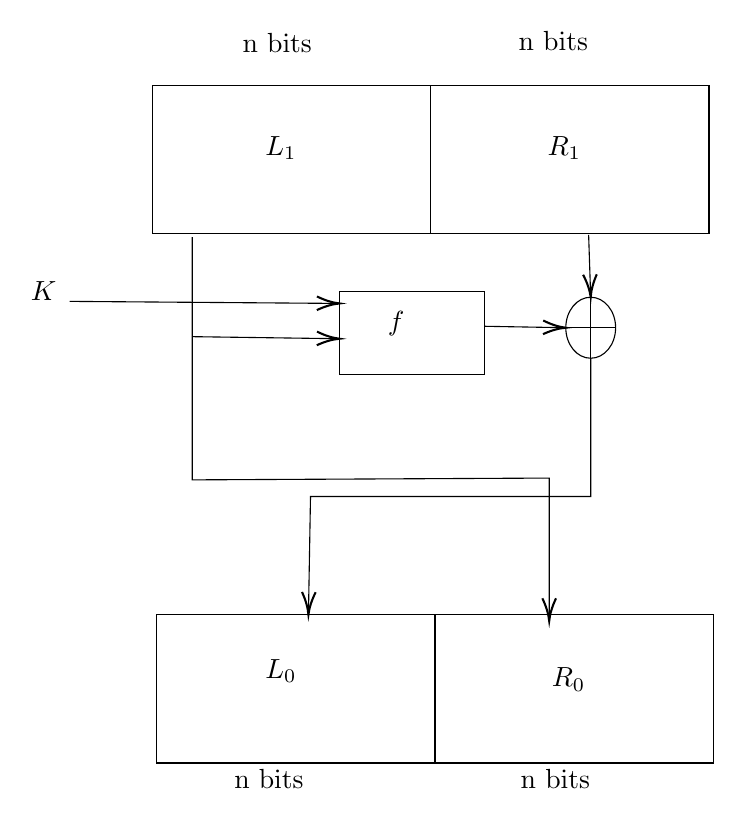
\begin{tikzpicture}[x=0.75pt,y=0.75pt,yscale=-1,xscale=1]
     
    \draw   (127,51.6) -- (261,51.6) -- (261,123) -- (127,123) -- cycle ;
    \draw   (261,51.6) -- (395,51.6) -- (395,123) -- (261,123) -- cycle ;
    \draw   (129,306.6) -- (263,306.6) -- (263,378) -- (129,378) -- cycle ;
    \draw   (263,306.6) -- (397,306.6) -- (397,378) -- (263,378) -- cycle ;
    \draw   (217,151) -- (287,151) -- (287,191) -- (217,191) -- cycle ; 
    \draw    (146,124.6) -- (146,241.6) -- (318.01,240.73) -- (318,307.6) ;
    \draw [shift={(318,309.6)}, rotate = 270] [color={rgb, 255:red, 0; green, 0; blue, 0 }  ][line width=0.75]    (10.93,-3.29) .. controls (6.95,-1.4) and (3.31,-0.3) .. (0,0) .. controls (3.31,0.3) and (6.95,1.4) .. (10.93,3.29)   ; 
    \draw   (326,168.3) .. controls (326,160.18) and (331.37,153.6) .. (338,153.6) .. controls (344.63,153.6) and (350,160.18) .. (350,168.3) .. controls (350,176.42) and (344.63,183) .. (338,183) .. controls (331.37,183) and (326,176.42) .. (326,168.3) -- cycle ; \draw   (326,168.3) -- (350,168.3) ; \draw   (338,153.6) -- (338,183) ; 
    \draw    (87,155.6) -- (215,156.58) ;
    \draw [shift={(217,156.6)}, rotate = 180.44] [color={rgb, 255:red, 0; green, 0; blue, 0 }  ][line width=0.75]    (10.93,-3.29) .. controls (6.95,-1.4) and (3.31,-0.3) .. (0,0) .. controls (3.31,0.3) and (6.95,1.4) .. (10.93,3.29)   ; 
    \draw    (146,172.6) -- (215,173.57) ;
    \draw [shift={(217,173.6)}, rotate = 180.81] [color={rgb, 255:red, 0; green, 0; blue, 0 }  ][line width=0.75]    (10.93,-3.29) .. controls (6.95,-1.4) and (3.31,-0.3) .. (0,0) .. controls (3.31,0.3) and (6.95,1.4) .. (10.93,3.29)   ;
    \draw    (287,167.6) -- (324,168.26) ;
    \draw [shift={(326,168.3)}, rotate = 181.03] [color={rgb, 255:red, 0; green, 0; blue, 0 }  ][line width=0.75]    (10.93,-3.29) .. controls (6.95,-1.4) and (3.31,-0.3) .. (0,0) .. controls (3.31,0.3) and (6.95,1.4) .. (10.93,3.29)   ; 
    \draw    (337,123.6) -- (337.93,151.6) ;
    \draw [shift={(338,153.6)}, rotate = 268.09] [color={rgb, 255:red, 0; green, 0; blue, 0 }  ][line width=0.75]    (10.93,-3.29) .. controls (6.95,-1.4) and (3.31,-0.3) .. (0,0) .. controls (3.31,0.3) and (6.95,1.4) .. (10.93,3.29)   ;
    \draw    (338,183) -- (338,249.6) -- (203,249.6) -- (202.04,304.6) ;
    \draw [shift={(202,306.6)}, rotate = 271.01] [color={rgb, 255:red, 0; green, 0; blue, 0 }  ][line width=0.75]    (10.93,-3.29) .. controls (6.95,-1.4) and (3.31,-0.3) .. (0,0) .. controls (3.31,0.3) and (6.95,1.4) .. (10.93,3.29)   ;
    
    \draw (180,75) node [anchor=north west][inner sep=0.75pt]   [align=left] {$L_1$};
    \draw (316,75) node [anchor=north west][inner sep=0.75pt]   [align=left] {$R_1$};
    \draw (318,331) node [anchor=north west][inner sep=0.75pt]   [align=left] {$R_0$};
    \draw (180,327) node [anchor=north west][inner sep=0.75pt]   [align=left] {$L_0$};
    \draw (239,159) node [anchor=north west][inner sep=0.75pt]   [align=left] {$f$};
    \draw (67,145) node [anchor=north west][inner sep=0.75pt]   [align=left] {$K$};
    \draw (169,25) node [anchor=north west][inner sep=0.75pt]   [align=left] {n bits};
    \draw (302,24) node [anchor=north west][inner sep=0.75pt]   [align=left] {n bits};
    \draw (165,380) node [anchor=north west][inner sep=0.75pt]   [align=left] {n bits};
    \draw (303,380) node [anchor=north west][inner sep=0.75pt]   [align=left] {n bits};
    \end{tikzpicture}
\end{center}
As it can be seen that the inverse of $f$ is not required in the decryption process. This means that it does not matter whether $f$ is invertible or not. In Fiestel networks, the round function may or may not be invertible.\\
\newline
It can be seen that one half of the plain text remains similar in the cipher text. However, only one round of implementation is shown. In general, there are multiple rounds and the whole message can be encrypted in later rounds.

\section{Iterated Block Cipher}
An Iterated Block Cipher is a block cipher involving the sequential repetition of an internal function (called the \textbf{Round Function}). The parameters includes \textbf{the number of rounds $r$, the block size $n$ and the round keys $K_i$ of length $l$ generated from the original secret key $K$.} 
A 3-round block cipher is shown below for example.
\begin{center}
    $f \rightarrow$ Round Function\\
    $P \rightarrow$ Plain Text Block\\
    $K \rightarrow$ Secret Key\\
\end{center}

\begin{center}
    \tikzset{every picture/.style={line width=0.75pt}}  
    \begin{tikzpicture}[x=0.75pt,y=0.75pt,yscale=-1,xscale=1]
    \draw   (189,99) -- (259,99) -- (259,139) -- (189,139) -- cycle ;
    \draw   (313,99) -- (383,99) -- (383,139) -- (313,139) -- cycle ;
    \draw   (432,99) -- (502,99) -- (502,139) -- (432,139) -- cycle ;
    \draw    (222,180) -- (222,141) ;
    \draw [shift={(222,139)}, rotate = 90] [color={rgb, 255:red, 0; green, 0; blue, 0 }  ][line width=0.75]    (10.93,-3.29) .. controls (6.95,-1.4) and (3.31,-0.3) .. (0,0) .. controls (3.31,0.3) and (6.95,1.4) .. (10.93,3.29)   ;
    \draw    (349,179) -- (349,140) ;
    \draw [shift={(349,138)}, rotate = 90] [color={rgb, 255:red, 0; green, 0; blue, 0 }  ][line width=0.75]    (10.93,-3.29) .. controls (6.95,-1.4) and (3.31,-0.3) .. (0,0) .. controls (3.31,0.3) and (6.95,1.4) .. (10.93,3.29)   ; 
    \draw    (466,179) -- (466,140) ;
    \draw [shift={(466,138)}, rotate = 90] [color={rgb, 255:red, 0; green, 0; blue, 0 }  ][line width=0.75]    (10.93,-3.29) .. controls (6.95,-1.4) and (3.31,-0.3) .. (0,0) .. controls (3.31,0.3) and (6.95,1.4) .. (10.93,3.29)   ;
    \draw    (136,118) -- (187,118.96) ;
    \draw [shift={(189,119)}, rotate = 181.08] [color={rgb, 255:red, 0; green, 0; blue, 0 }  ][line width=0.75]    (10.93,-3.29) .. controls (6.95,-1.4) and (3.31,-0.3) .. (0,0) .. controls (3.31,0.3) and (6.95,1.4) .. (10.93,3.29)   ; 
    \draw    (260,118) -- (311,118.96) ;
    \draw [shift={(313,119)}, rotate = 181.08] [color={rgb, 255:red, 0; green, 0; blue, 0 }  ][line width=0.75]    (10.93,-3.29) .. controls (6.95,-1.4) and (3.31,-0.3) .. (0,0) .. controls (3.31,0.3) and (6.95,1.4) .. (10.93,3.29)   ;
    \draw    (383,118) -- (431,118) ;
    \draw [shift={(433,118)}, rotate = 180] [color={rgb, 255:red, 0; green, 0; blue, 0 }  ][line width=0.75]    (10.93,-3.29) .. controls (6.95,-1.4) and (3.31,-0.3) .. (0,0) .. controls (3.31,0.3) and (6.95,1.4) .. (10.93,3.29)   ;
    \draw    (503,117) -- (551,117) ;
    \draw [shift={(553,117)}, rotate = 180] [color={rgb, 255:red, 0; green, 0; blue, 0 }  ][line width=0.75]    (10.93,-3.29) .. controls (6.95,-1.4) and (3.31,-0.3) .. (0,0) .. controls (3.31,0.3) and (6.95,1.4) .. (10.93,3.29)   ;
    \draw (211,181) node [anchor=north west][inner sep=0.75pt]   [align=left] {$K_1$};
    \draw (338,180) node [anchor=north west][inner sep=0.75pt]   [align=left] {$K_2$};
    \draw (455,180) node [anchor=north west][inner sep=0.75pt]   [align=left] {$K_3$};
    \draw (214,110) node [anchor=north west][inner sep=0.75pt]   [align=left] {$f$};
    \draw (341,108) node [anchor=north west][inner sep=0.75pt]   [align=left] {$f$};
    \draw (459,109) node [anchor=north west][inner sep=0.75pt]   [align=left] {$f$};
    \draw (113,109) node [anchor=north west][inner sep=0.75pt]   [align=left] {P};
    \draw (557,107) node [anchor=north west][inner sep=0.75pt]   [align=left] {C};
    \end{tikzpicture}
\end{center}

\begin{center}
    C $\rightarrow$ cipher text\\
    $G(K) \rightarrow K_1, K_2, K_3$ (round keys)\\ 
\end{center}
The function G, knows as \textbf{Key Scheduling Function} generates the round keys by taking the secret key as input.

\section{One Time Padding}
One Time Padding (OTP) provides perfect secrecy under some conditions.\\
\newline
\textbf{Encryption: }
\begin{center}
    P $\rightarrow$ Plain Text\\
    K $\rightarrow$ Secret Key\\
    $Enc(P, K) = P \oplus K = C$\\
    $\oplus \rightarrow $ xor operation\\
\end{center}
\textbf{Decryption: }
\begin{center}
    $Dec(C, K) = C \oplus K = P$\\
\end{center}
The conditions under which OTP provides perfect secrecy are as follows:
\begin{enumerate}
    \item The secret key K cannot be used to encrypt two messages, that is, the key can not be reused.
    \item The length of key must be greater than or equal to the length of message.
    \item Key K is uniformly selected from the key space.
\end{enumerate}
Stream Cipher is a generalisation of OTP which does not provide perfect secrecy.
\end{document}
